\documentclass[conference]{IEEEtran}

\usepackage[utf8]{inputenc}
\usepackage[english]{babel}
\usepackage{graphicx}
\usepackage{natbib}
\usepackage{url} % Required for proper URL formatting in references
\usepackage{tikz}
\usetikzlibrary{positioning,arrows.meta}

\begin{document}

\title{Implementing 'Gordon': A NAO Robot Receptionist to Enhance Efficiency in Critical Services Using Choregraphe and Python}

\author{
\IEEEauthorblockN{
        Diana Milligan\IEEEauthorrefmark{1},
        Filip Hanuš\IEEEauthorrefmark{1},
        Harry Williams\IEEEauthorrefmark{1},\\
        Jack Thompson\IEEEauthorrefmark{1},
        Natalie Leung\IEEEauthorrefmark{1}
}
\IEEEauthorblockA{
        \IEEEauthorrefmark{1}School of Engineering, College of Art, Technology and Environment,\\ University of the West of England, Bristol, UK\\
        Email: diana2.milligan, filip2.hanus, harry4.williams, jack2.ould, wing7.leung\}@live.uwe.ac.uk}
}

\maketitle

\begin{abstract}

This paper presents what is in this abstract. 

\end{abstract}

\begin{IEEEkeywords}

NAO Robot, Human Robot Interaction.

\end{IEEEkeywords}

\section{Distribution of Work} This project has been equally distributed to and completed by the authors of this report.

\section{Introduction and Related Works}

The purpose of this project is to use a NAO robotic platform to effectively perform a task that requires direct interaction with humans. 
There are various metrics that can be used to quantify the success of such a system, but as a broader definition an effective system 
should be able to receive and convey relevant information to an untrained user to achieve a wider goal.

A task that lends itself to this project brief is a reception environment, particularly in a medical setting. According to 
Mallorie \cite{mallorie2024}, managerial staff shortages within the NHS has pushed clinical staff to spend more time on administrative task over 
patient-facing care. To effectively reduce staffing requirements and thus make the running of medical centers less resource intensive, robotic 
systems can be integrated to alleviate the bulk of repetitive tasks. A good low-risk opportunity for this kind of integration is within a 
receptionist role where any possible errors are of a significantly lower severity than other roles (e.g. medical diagnosis and treatment).
A study conducted by Sutherland et al. \cite{Sutherland2019} tested the concept of a robotic receptionist for medical purposes, concluding that the robot displayed a 
"professional level of friendliness" that made it suited the role. However, the testing used Wizard-of-Oz methodologies with the robot only 
used as the interface between a user and a remote operator. Had all the behaviours been generated by the robot, there could have been 
a significant difference in how it was perceived by users.

Methods to create a sense of authority for robots have been explored through many different ways, many of which can be implemented within 
this project. Rae et al. \cite{Rae2013} explored the effect of height on robotic telepresence systems, concluding that a shorter "leader" was less persuasive 
for a the human follower. As well as the robot's stature, Rossi (need citation) found that contextual information such as the location of an interaction 
helped users infer the robot’s role.

Appearance has been argued to be a less important factor by Natarajan and Gombolay (need citation) who tested a variety of different variables for artificial agents, with 
behaviour being "the most significant factors in predicting the trust and compliance with the robot" rather 
than physical appearance. A Nao platform has been used by Cormier et al. \cite{cormier2013v2} to test the limitations of such compliance, finding that users would 
refuse to follow challenging orders from a robot if factors such as perceived intelligence or professionalism were compromised.

\section{Scope and Assumptions} In Scope:
\begin{itemize}
        \item Begin client/robot interaction with a waving motion
        \item Greet client and recognise which staff member they have an appointment with
        \item NAO finds the appointment and emails staff that the client has arrived
        \item Create natural gestures that NAO performs during client interaction    
\end{itemize}

Out of Scope:
\begin{itemize}
        \item Exploring alternative robots
        \item System is not connected to a database of appointments 
\end{itemize}

Assumptions:
\begin{itemize}
        \item Interactions will converse in British English only.
        \item NAO will be positioned out of reach from client users
        \item NAO will always be powered on
\end{itemize}

\section{Technical Implementation}

Below is the technical implementation of the project, starting with the high level description of the state machine with the final state diagram. This is then
followed by the more deliberate description of the states and the transitions between them. The sentences spoken by the robot are then detailed,
followed by the code overview. 

\begin{figure}
  \centering
  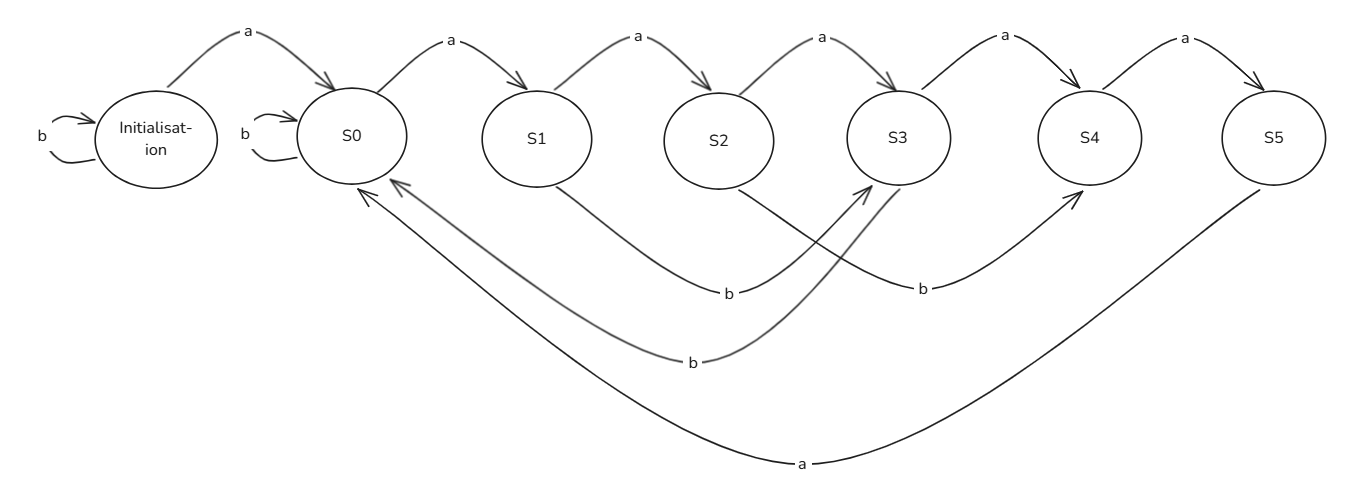
\includegraphics[width=.9\linewidth]{Final state diagram.png}
  \caption{Final state diagram}
  \label{Final state diagram}
\end{figure}

\subsection{State Machine Description}

\subsubsection{System Start}
\paragraph{Entry Condition:}
\mbox{}\\
The robot/system is powered on or reset. This is the initial state.

\paragraph{Actions:}
\begin{itemize}
  \item Immediately triggers \textbf{Face Detection}, looking for any faces in view.
  \item Checks whether the \emph{number of faces} has changed (i.e., a new face appears).
  \item If a new face is detected, the system attempts to \emph{Learn face (employee)}. If learning is successful, it proceeds with a \emph{Success message}; if unsuccessful, it gives a \emph{Failure message}.
\end{itemize}

\paragraph{Transitions:}
\begin{itemize}
  \item Both the \emph{success} and \emph{failure} learning branches eventually converge and transition to \textbf{State 0}. This is in order to prevent getting stuck due to NAO's technical problems.
\end{itemize}

\begin{figure}
    \centering
    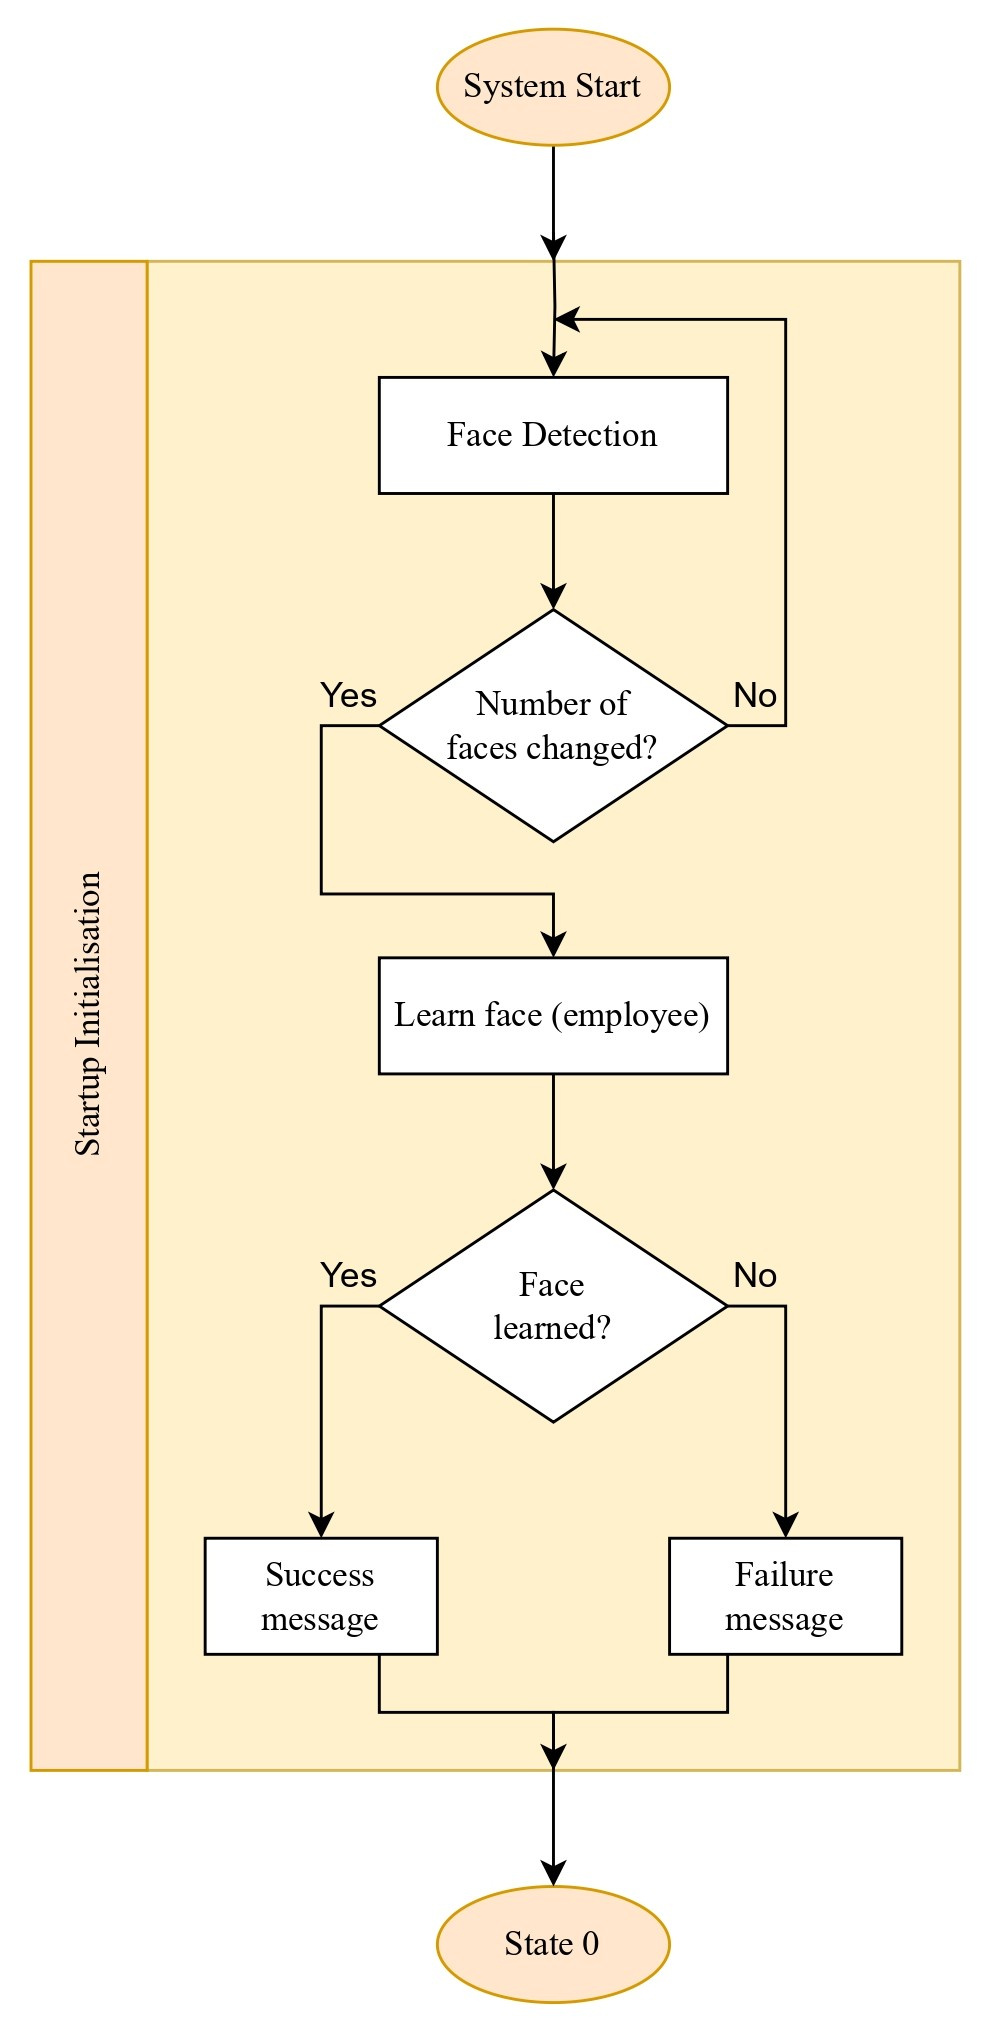
\includegraphics[width=.6\linewidth]{Startup Initialisation.jpg}
    \caption{Startup Initialisation}
    \label{Startup Initialisation}
\end{figure}

\subsubsection{State 0}
\paragraph{Entry Condition:}
\mbox{}\\
The machine enters this state after finishing the initial face-detection/learning process.

\paragraph{Actions:}
\begin{itemize}
  \item Continuously \emph{reads webcam input}.
  \item Monitors for a \emph{wave} via MediaPipe.
\end{itemize}

\paragraph{Transitions:}
\begin{itemize}
  \item If a wave is detected, perform \emph{Action: Wave back} and move to \textbf{State 1}.
  \item If no wave is detected, remain in \textbf{State 0} and continue monitoring.
\end{itemize}

\begin{figure}
    \centering
    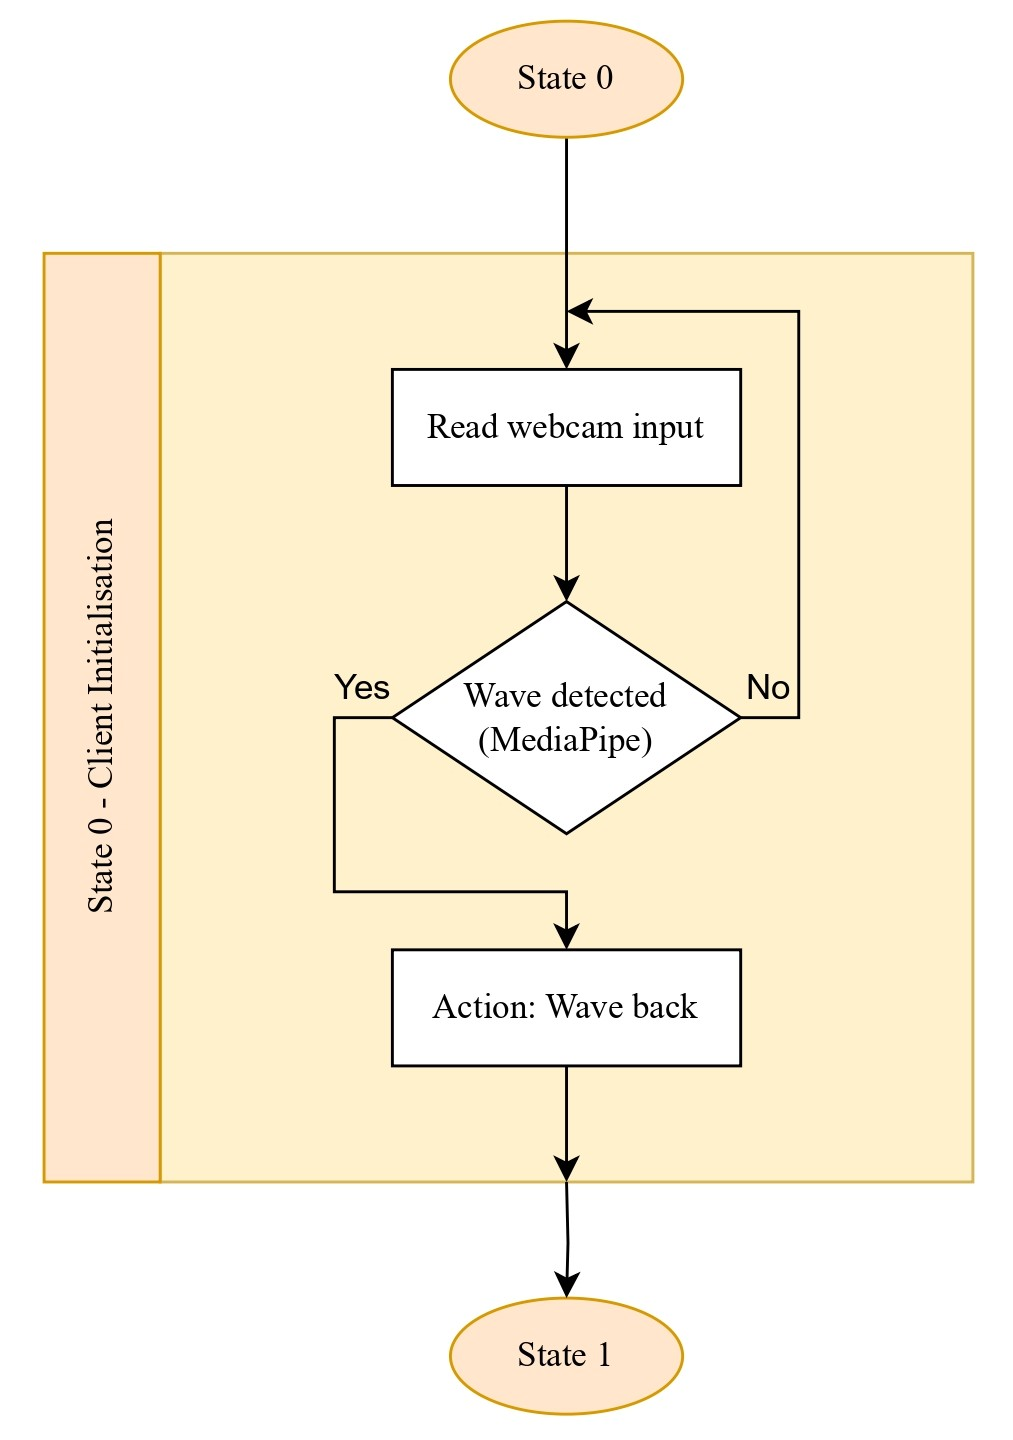
\includegraphics[width=.6\linewidth]{State 0 - Client Initialisation.jpg}
    \caption{State 0 - Client Initialisation}
    \label{State 0 - Client Initialisation}
\end{figure}

\subsubsection{State 1}
\paragraph{Entry Condition:}
\mbox{}\\
A wave has been detected in \textbf{State 0}, triggering the move here (``Client Appointment Initialisation'').

\paragraph{Actions:}
\begin{itemize}
  \item Asks the user if they have an appointment.
  \item Performs \emph{Speech Recognition} to capture their answer.
  \item Checks if the answer is ``yes'' or ``no''.
\end{itemize}

\paragraph{Transitions:}
\begin{itemize}
  \item If \emph{yes}, transition to \textbf{State 2} (handle appointment details).
  \item If \emph{no}, transition to \textbf{State 3} (offer human assistance).
\end{itemize}

\begin{figure}
    \centering
    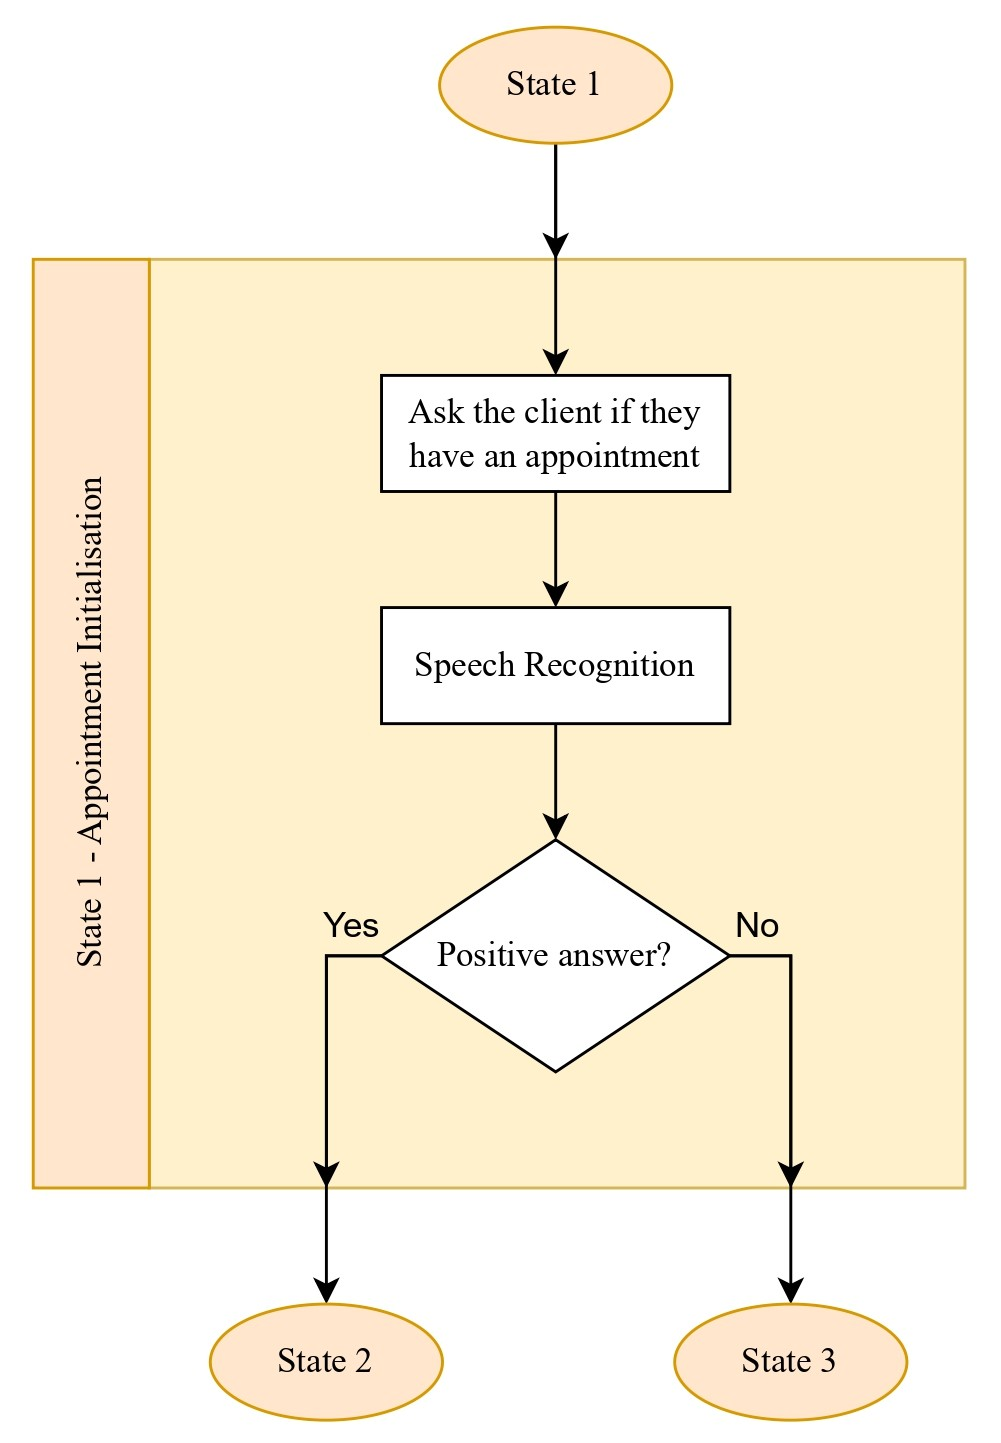
\includegraphics[width=.6\linewidth]{State 1 - Appointment Initialisation.jpg}
    \caption{State 1 - Appointment Initialisation}
    \label{State 1 - Appointment Initialisation}
\end{figure}

\subsubsection{State 2}
\paragraph{Entry Condition:}
\mbox{}\\
User has indicated they do have an appointment.

\paragraph{Actions:}
\begin{itemize}
  \item Prompts for the name of the staff member or the confirmation number.
  \item Uses \emph{Speech Recognition}, then checks if the provided information is found in the database.
  \item Keeps track of the number of failed attempts.
\end{itemize}

\paragraph{Transitions:}
\begin{itemize}
  \item If the name or confirmation number is valid, \emph{nod head} and transition to \textbf{State 4} (staff notification).
  \item If it is invalid, increment the failure count. If failures exceed 2, \emph{shake head} and move to \textbf{State 3}.
\end{itemize}

\begin{figure}
    \centering
    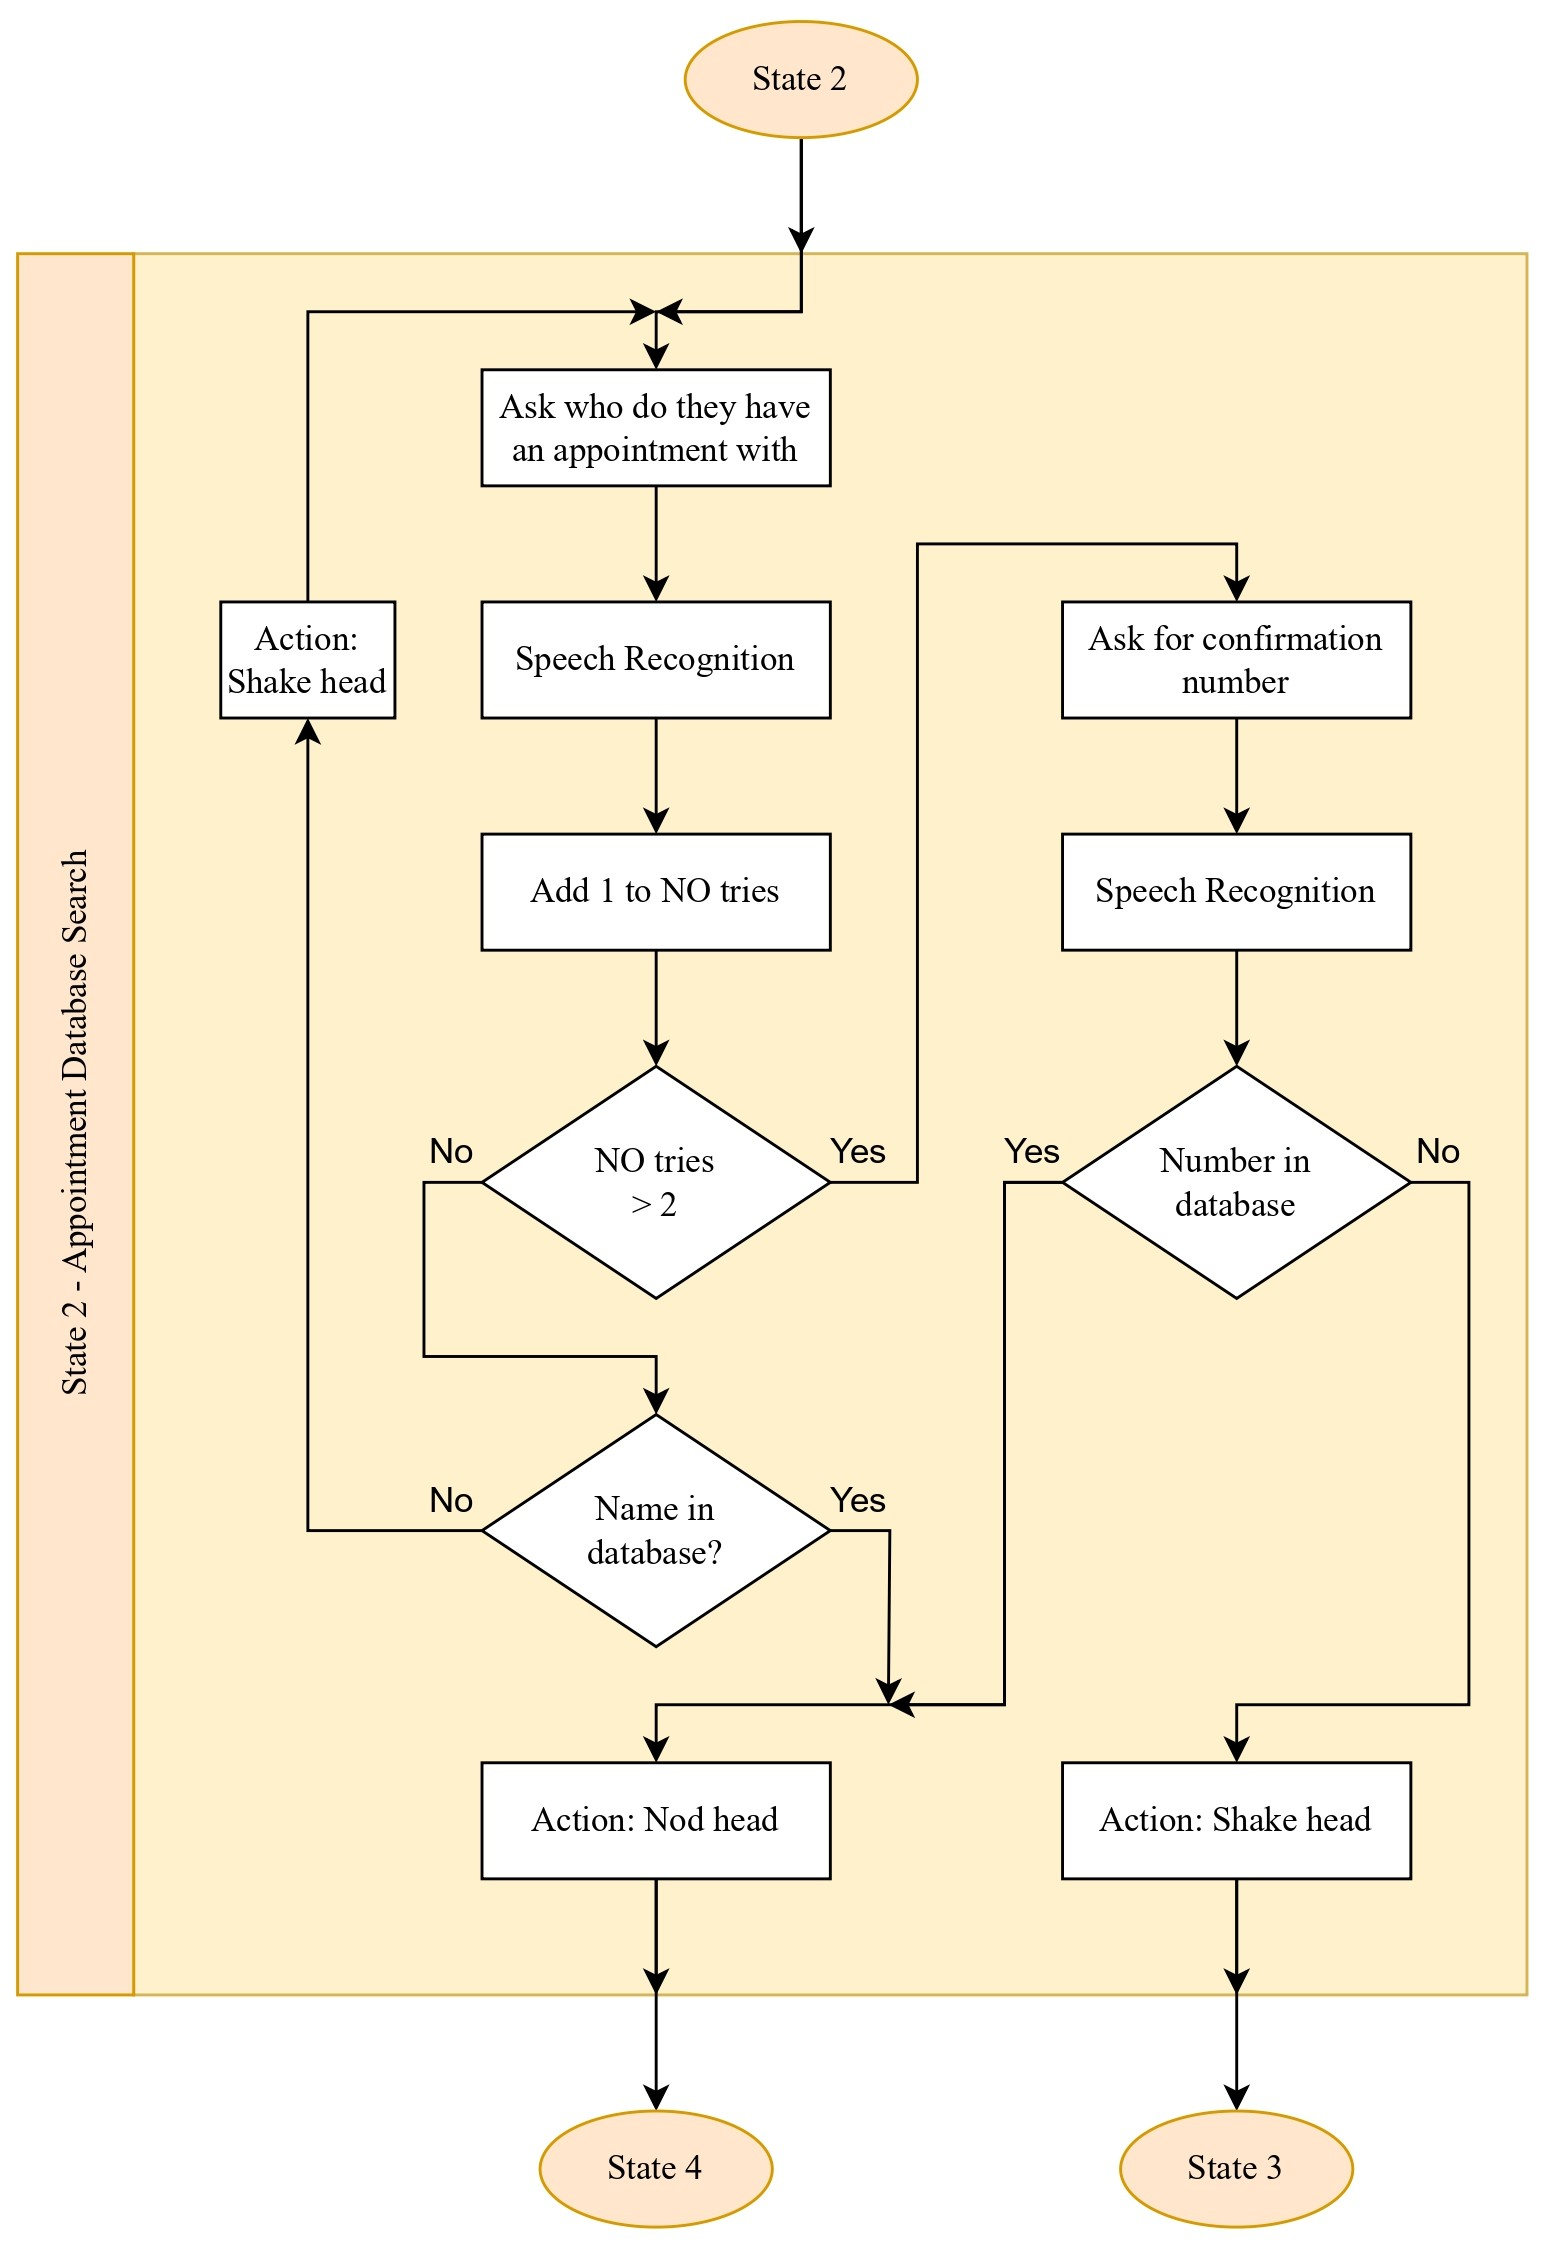
\includegraphics[width=.6\linewidth]{State 2 - Appointment Database Search.jpg}
    \caption{State 2 - Appointment Database Search}
    \label{State 2 - Appointment Database Search}
\end{figure}

\subsubsection{State 3}
\paragraph{Entry Condition:}
\mbox{}\\
Either the user said they have no appointment (from State 1) or they exceeded failures in State 2.

\paragraph{Actions:}
\begin{itemize}
  \item Asks the user if they would like to call a human staff member.
  \item Performs \emph{Speech Recognition} and checks if the answer is positive or negative.
\end{itemize}

\paragraph{Transitions:}
\begin{itemize}
  \item If \emph{yes}, \emph{nod head} and proceed to \textbf{State 4}.
  \item If \emph{no}, \emph{shake head} and return to \textbf{State 0}.
\end{itemize}

\begin{figure}
    \centering
    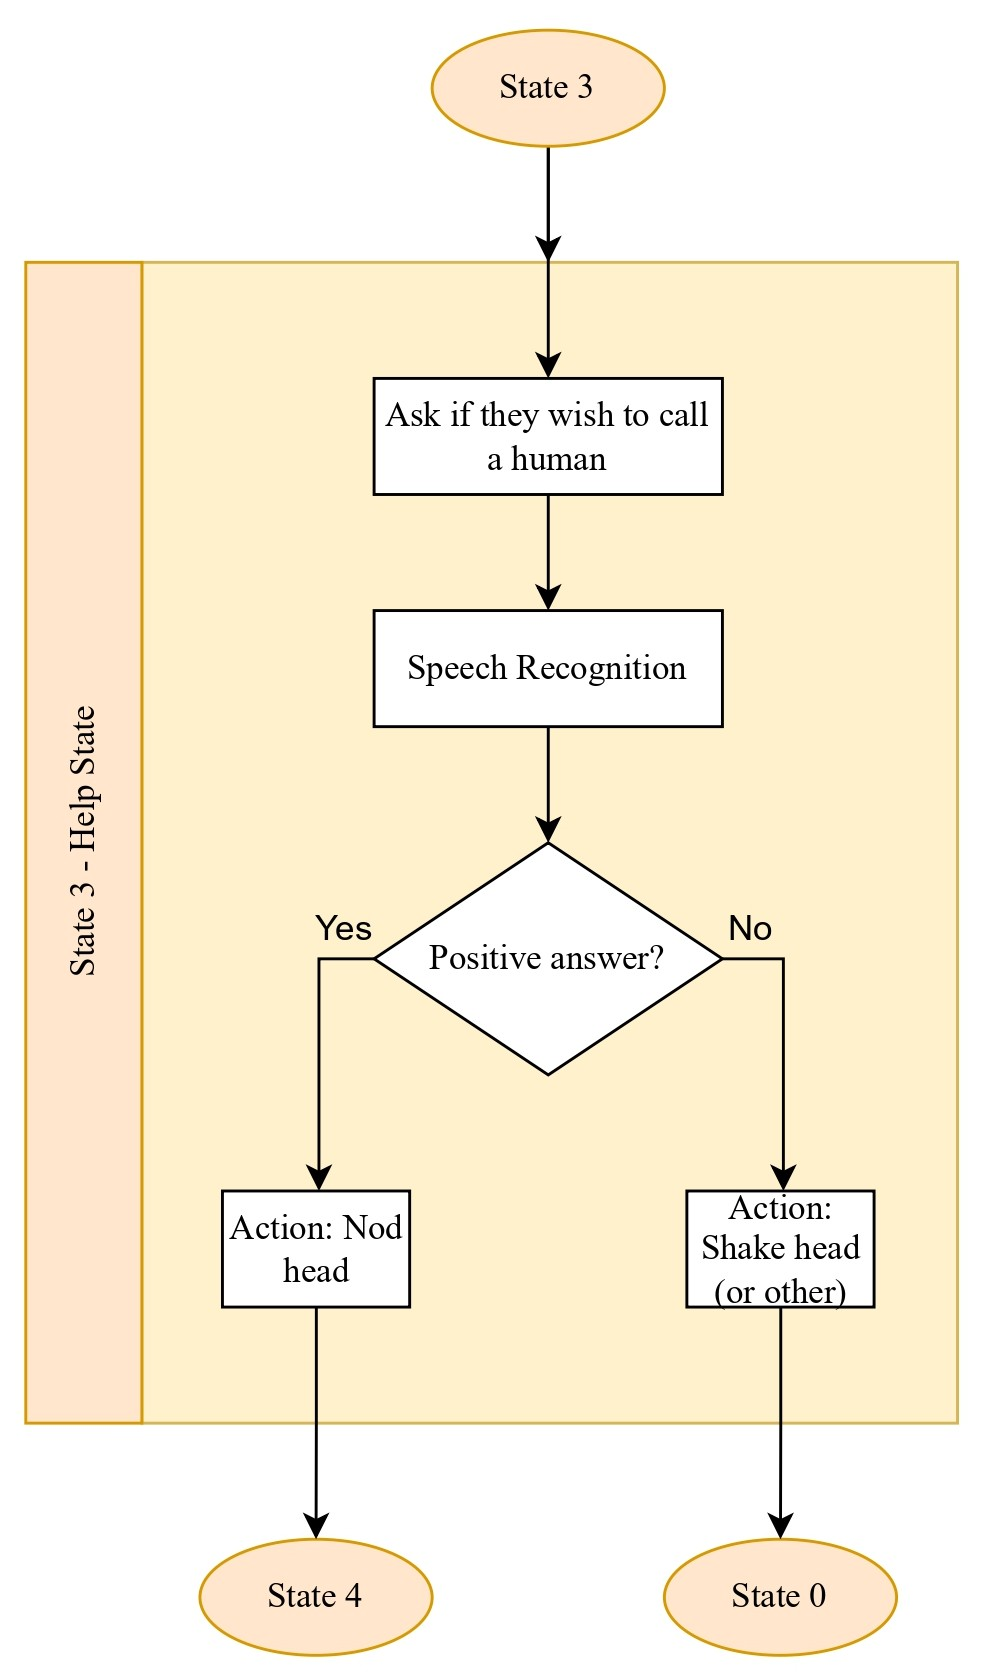
\includegraphics[width=.6\linewidth]{State 3 - Help State.jpg}
    \caption{State 3 - Help State}
    \label{State 3 - Help State}
\end{figure}

\subsubsection{State 4}
\paragraph{Entry Condition:}
\mbox{}\\
Indicates the system must notify staff (arrived from State 2 or State 3).

\paragraph{Actions:}
\begin{itemize}
  \item Performs \emph{Action: Computer Glance}, then sends an email to the specified staff member.
  \item Announces that staff has been notified.
\end{itemize}

\paragraph{Transitions:}
\begin{itemize}
  \item Moves on to \textbf{State 5} after notifying staff and confirming the message was sent.
\end{itemize}

\begin{figure}
    \centering
    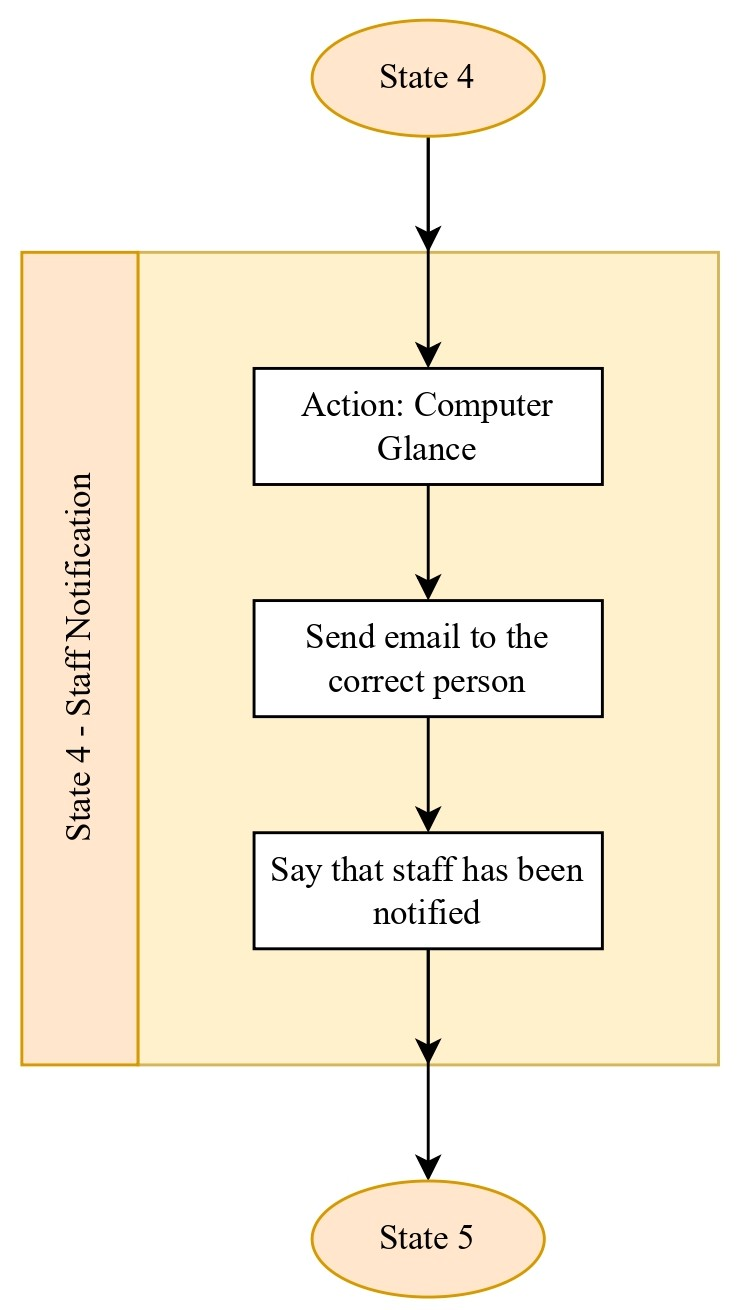
\includegraphics[width=.6\linewidth]{State 4 - Staff Notification.jpg}
    \caption{State 4 - Staff Notification}
    \label{State 4 - Staff Notification}
\end{figure}

\subsubsection{State 5}
\paragraph{Entry Condition:}
\mbox{}\\
Staff have been notified that a visitor is waiting.

\paragraph{Actions:}
\begin{itemize}
  \item Informs the user that staff will arrive soon.
  \item Asks the user to rate their experience, capturing input via \emph{Speech Recognition}.
  \item Runs \emph{Sentiment Analysis} to interpret the feedback.
  \item Thanks the user for their feedback.
  \item Monitors for any change in faces to detect if staff has arrived.
\end{itemize}

\paragraph{Transitions:}
\begin{itemize}
  \item If the staff’s face is now recognised, the system \emph{waves} and returns to \textbf{State 0}, ready for the next interaction cycle.
\end{itemize}

\begin{figure}
    \centering
    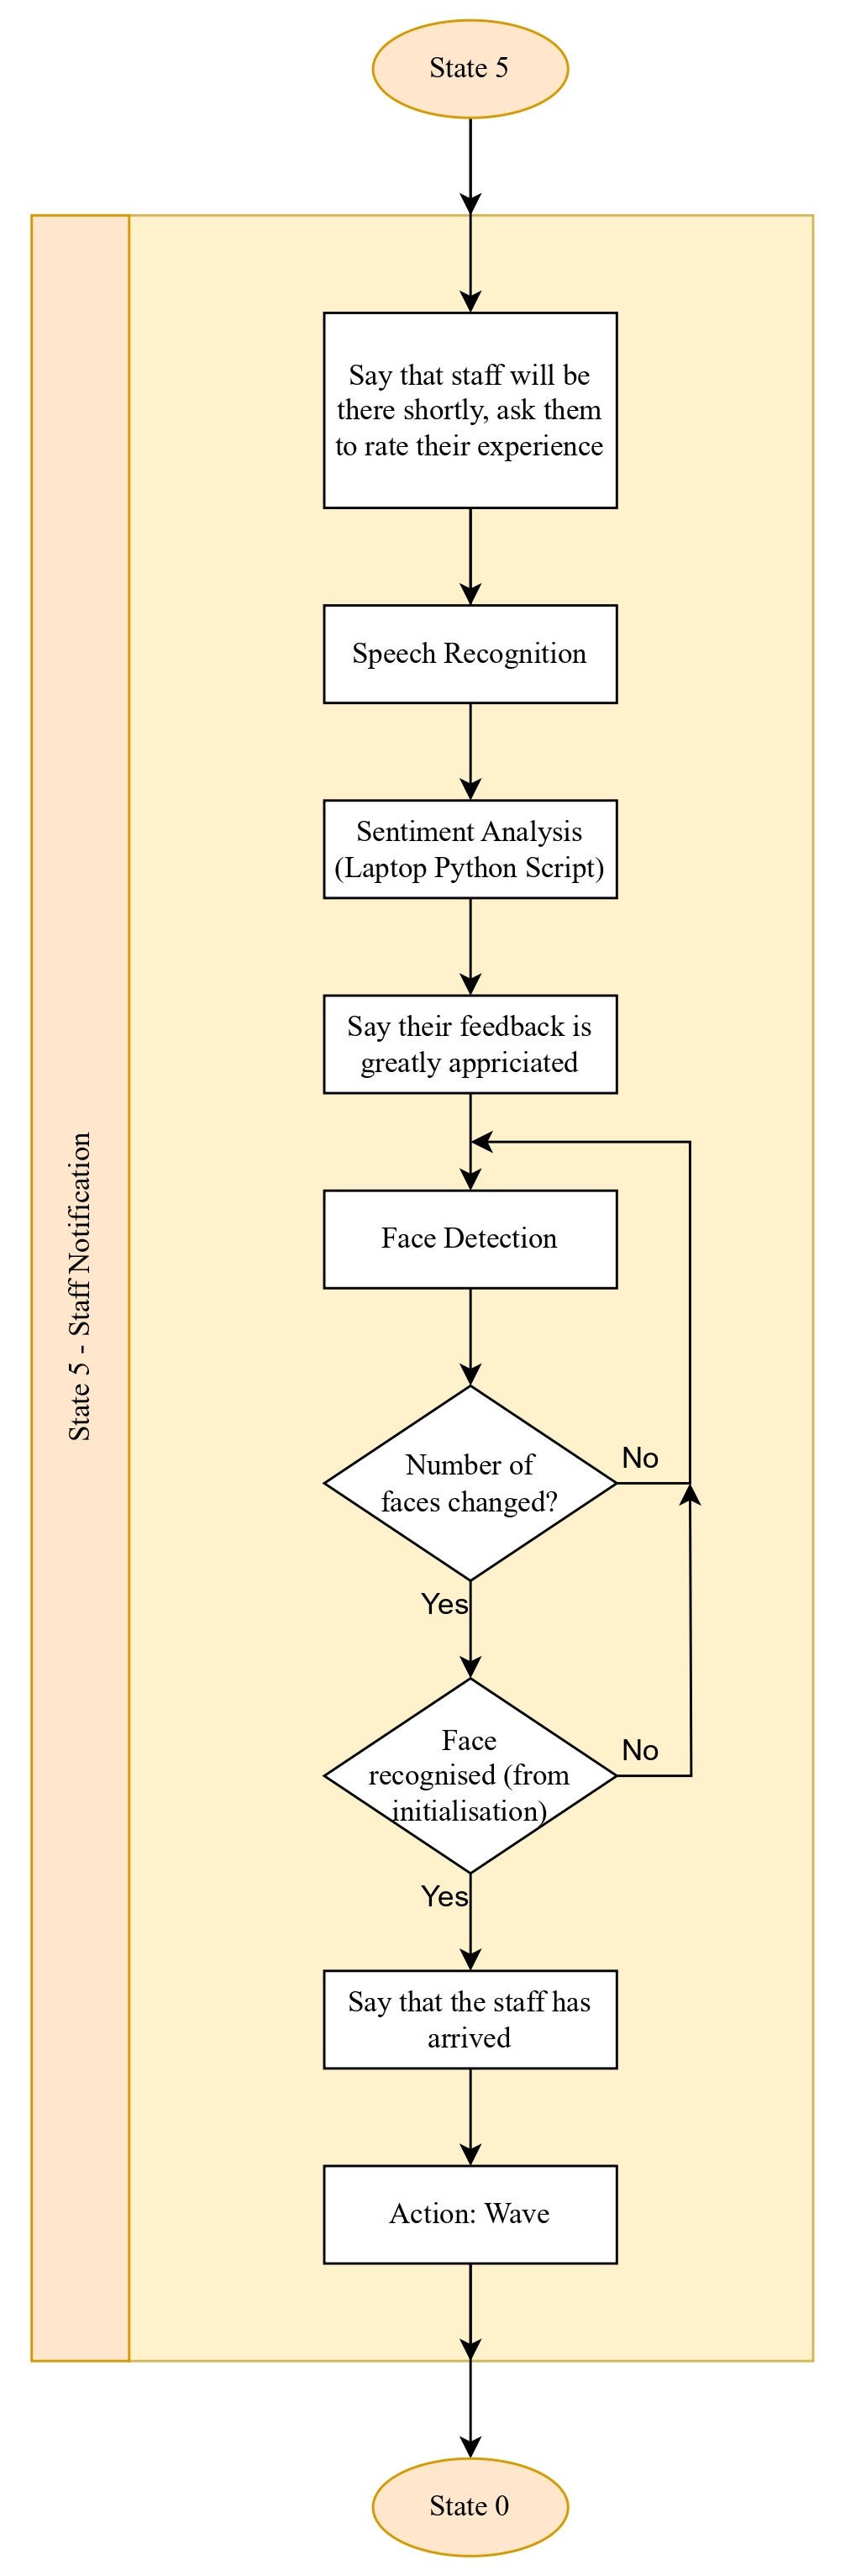
\includegraphics[width=.6\linewidth]{State 5 - Staff Notification.jpg}
    \caption{State 5 - Staff Notification}
    \label{State 5 - Staff Notification}
\end{figure}


\subsection{Sentences Spoken by the Robot}

The robot has several states (\textbf{State 0} to \textbf{State 5}), each with characteristic announcements or prompts. Below are samples of the main utterances (also visible in the previous subsection):

\begin{itemize}
  \item \textbf{State 1}:
    \begin{itemize}
      \item \texttt{``Hi, my name is Gordon, do you have an appointment?''} \\
    \end{itemize}

  \item \textbf{State 2}:
    \begin{itemize}
      \item \texttt{``Who do you have an appointment with?''} \\
            Prompts for the staff member’s name.
      \item \texttt{``May I ask for your confirmation number?''}
      \item \texttt{``Sorry, didn't catch that''} \\
            If speech recognition is unclear or fails.
      \item \texttt{``I've got you''} \\
            If a matching name/number was found.
      \item \texttt{``That is not in our database''} \\
            If no match is found for either the name or number.
    \end{itemize}

  \item \textbf{State 3}:
    \begin{itemize}
      \item \texttt{``Do you want to call a human?''}
    \end{itemize}

  \item \textbf{State 4}:
    \begin{itemize}
      \item \texttt{``I have sent an email to the member of staff.''} \\
    \end{itemize}

  \item \textbf{State 5}:
    \begin{itemize}
      \item Additional prompts about staff arrival and requesting user feedback.
    \end{itemize}
\end{itemize}



\subsection{Code Overview}

The project employs external webcamera vision system for hand gesture detection (wave detection, rude gestures from angry customers), integrating OpenCV and MediaPipe.

\subsubsection{Main Components}
\begin{itemize}
  \item \textbf{SimpleServer Class:} 
    \begin{itemize}
      \item Handles TCP socket communication, accepting client connections and sending messages.
      \item Manages concurrency using threads and locks to ensure safe communication between the robot and external clients.
    \end{itemize}
  \item \textbf{\texttt{detectWave} Function:} 
    \begin{itemize}
      \item Utilises OpenCV to capture video frames and MediaPipe to process hand landmarks.
      \item Detects waving gestures and rude gestures based on the relative positions of hand landmarks.
      \item Sends corresponding signals (e.g., ``Wave'', ``Rude'') to the connected client (NAO) via the server.
    \end{itemize}
  \item \textbf{\texttt{handle\_client} Function:} 
    \begin{itemize}
      \item Receives text input from the client socket.
      \item Analyses the sentiment of the received text using NLTK's VADER SentimentIntensityAnalyzer.
      \item Sends back a sentiment response (Positive/Negative/Neutral) to the client.
    \end{itemize}
  \item \textbf{\texttt{image\_processing} Function:} 
    \begin{itemize}
      \item Preprocesses video frames by flipping and converting color spaces for MediaPipe processing.
    \end{itemize}
\end{itemize}

\subsubsection{Interaction Diagram}

\begin{figure}[!ht]
\centering
\resizebox{0.9\columnwidth}{!}{
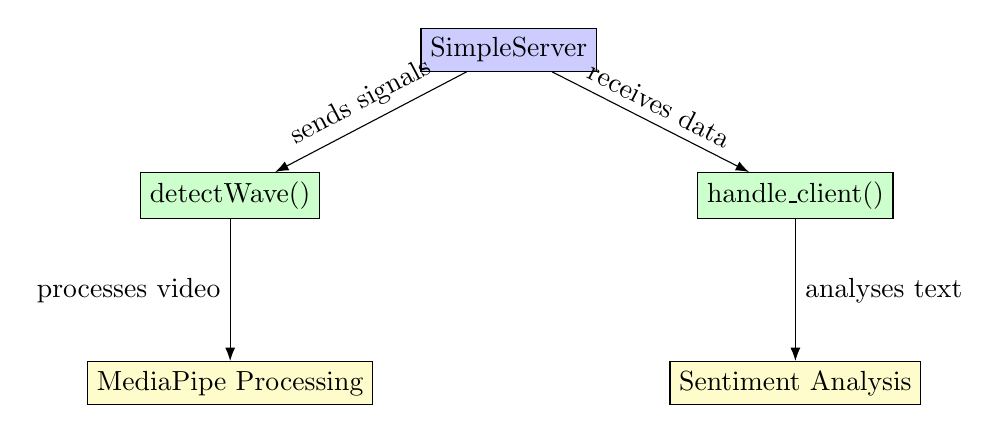
\begin{tikzpicture}[node distance=1.8cm, auto, >=Latex]
  % Nodes
  \node[rectangle, draw, fill=blue!20] (server) {SimpleServer};
  \node[rectangle, draw, fill=green!20, below left=of server] (detectWave) {detectWave()};
  \node[rectangle, draw, fill=green!20, below right=of server] (handleClient) {handle\_client()};
  \node[rectangle, draw, fill=yellow!20, below=of detectWave] (mediapipe) {MediaPipe Processing};
  \node[rectangle, draw, fill=yellow!20, below=of handleClient] (sentiment) {Sentiment Analysis};

  % Arrows
  \draw[->] (server) -- node[midway, above, sloped] {sends signals} (detectWave);
  \draw[->] (server) -- node[midway, above, sloped] {receives data} (handleClient);
  \draw[->] (detectWave) -- node[midway, left] {processes video} (mediapipe);
  \draw[->] (handleClient) -- node[midway, right] {analyses text} (sentiment);
\end{tikzpicture}
}
\caption{System interaction flow diagram showing main components and their relationships}
\label{fig:interaction-diagram}
\end{figure}

\subsubsection{System Workflow}

\begin{enumerate}
  \item \textbf{Initialisation:} The main program creates a \texttt{SimpleServer} instance, waiting for a client connection.
  \item \textbf{Wave Detection Loop:} Once connected, the system enters a loop calling \texttt{detectWave()}, processing camera frames to detect gestures.
  \item \textbf{Signal Communication:} Upon detecting a gesture, \texttt{detectWave()} spawns a thread to send the appropriate signal (e.g., "Wave", "Rude") via the server.
  \item \textbf{Client Handling:} Simultaneously, \texttt{handle\_client()} listens for incoming text data from the client, processes sentiment, and sends back a response.
\end{enumerate}

\subsection{GitHub} A shared GitHub housed README files, NAO scripts, and LaTeX documentation for report writing. Branches broke down project tasks and features, whilst version control assisted with project collaboration and testing. See Appendix for supporting GitHub documentation.

\subsection{Design Rationale} NAO was placed at eye-level to improve authority and user engagement,
as recommended by Rae et al.\cite{Rae2013}. This aligns with Sutherland et al.\cite{Sutherland2019}, who demonstrated the advantages of
a robotic receptionist in clinical settings. This project builds upon their Wizard-of-Oz study by enabling NAO to generate all behaviours independently.

\subsection{Contingency Measures} In practice, user trust decreases sharply when robots show consistent errors, as reported by Bistolfi~\cite{Bistolfi2022}.
Therefore, clear fallback steps were embedded:
\begin{itemize}
        \item If the appointment check-in fails, staff are alerted via email.
\end{itemize}

\subsection{Hazard Mitigation} Following a risk assessment, a highlighted safety concern of NAO are the ‘pinch points’ during robotic movements. To avoid physical contact, NAO will be placed behind a desk and out of reach from the user.

\section{HRI Dialogue Example}

\textit{[User wave detected]}
Gordon: Hi! My name is Gordon. Do you have an appointment?
User: Yes, I do.
Gordon: Who do you have an appointment with?
User: [unrecognisable mumbling]
Gordon: Sorry, didn't catch that.
User: I have an appointment with Bob.
\textit{[Gordon checks the database for an employee called Bob. Bob doesn’t exist.]}
Gordon: May I ask for your confirmation number?
User: My appointment number is 4.
\textit{[Gordon checks the database for a matching confirmation number. Confirmation number exists.]}
Gordon: I have got you.
\textit{[Gordon sends staff member an email]}
Gordon: I have sent an email to the member of staff. Someone will be with you shortly.  In the meantime, how would you rate your experience with me on a scale of 1 to 10?
User: 10! Your service was fantastic.
Gordon: Your feedback is greatly appreciated, thank you. 
\textit{[Gordon detects the staff member walking in]}
Gordon: Our staff is here to help you. Bye.

Scenario: A patient checks in with NAO. The user has an appointment with a staff member, however, that staff member does not exist, NAO prompts the user for their confirmation number. NAO locates the appointment and sends an email to the correct employee. Whilst the user is waiting, NAO asks for user feedback. NAO detects the staff member and announces their arrival.

This scripted scenario highlights two particular failure points anticipated in the system design. Firstly, NAO cannot recognise the user’s first response detailing who they have an appointment with. Secondly, the user mistakenly provides the name of someone who does not work there.  The system is designed to allow a maximum of two attempts to find the employee, then the user is prompted to provide a confirmation number. If the appointment is located, the script follows as above. Alternatively, if the appointment cannot be found, NAO can follow an expanded script asking if the user would like to speak with a human and emails the manager to assist. NAO can determine these failure points as the Python script contains a predetermined list of the employees. NAO listens for these predetermined words. If the user fails to correctly articulate an employee’s name from the predetermined list, NAO will then proceed with the contingencies put in place as part of the system design. To maintain a positive user experience, the user will only be prompted to repeat themselves once, beyond this, human intervention will be offered to avoid user frustrations with the robot. 


\section{Future Work}Facial recognition was planned and developed but was not able to be featured in the final testing due to 
technical difficulties. Future work on this project would include and expand upon this capability as recognising (and potentially 
analysing) individuals vastly increases the functionality and perceived intelligence of the system.

To improve the quality of the current conversations, integrating a more robust NLP algorithm increases the likelihood that the NAO 
robot correctly understands the user’s intent from a single output. Currently, any output outside of expected values is considered 
an error and handled accordingly. NLP allows more unexpected inputs to be parsed for key information that otherwise would’ve been 
missed, directing the robot towards a more appropriate response.

While these improvements would improve the technology, extensive user testing (especially within the intended medical space) is the 
best way to understand the system's shortcomings and improve accordingly.


\section{Discussion}
In general, HRI is an element that should be considered early in the design stage, allowing engineers to understand limitations of the system and manage user expectation.
\subsection{Plan vs implementation}

The initial system design included features such as face recognition and Natural Language Processing (NLP); however, these were unsuccessful during the final implementation. 

The face recognition intended to detect and store staff members' faces in the initialisation state. This would be utilised later (in state 5), where the NAO robot could recognise the arrival of the staff member and introduce them to the patiently waiting patient. The purpose was to create a more intelligent and cohesive user experience. Whilst the face detection was designed and implemented, it only proved successful one-in-ten attempts. This was due to technical difficulties with the face recognition software in Choregraphe. Adding delay and loops for testing purposes did not solve the problem. To ensure face recognition did not stop the execution of the remaining system, a message would announce ‘detection face successful’ or ‘detection face failed’ and either output would trigger the next state. Integrating other software is a consideration of future improvements.

NLP was again designed but was not ultimately implemented in the final system. During testing, NLP provided promising results; however, the complex sentences were difficult for NAO to recognise and perform speech-to-text functionality. This is due to the limitation of NAO’s hardware and speech recognition in Choregraphe. Various voices were used but ultimately could not be integrated in the implementation. NLP would have benefited the system for a more complex interaction with the user. It would have processed complicated text and understand the abstract of ideas, such as analysing sentiment of the user feedback. Speech recognition for complex input was considered to assist NLP; however, time limitations and the subscription required for implementation prevented its execution.

Whilst these methods were a bonus to this project, the system was still able to incorporate gesture detection to detect a wave and used the text-to-speech (TTS) and speech-to-text (STT) functionalities within Choregraphe to converse with the user. 



\subsection{Project Limitations}

\begin{enumerate} 
        \item \textbf{Speech recognition constraints.} NAO struggles with various accents and complex sentences. Improvements could be made by integrating more sophisticated speech recognition software like Microsoft Azure or Google Speech-to-Text. Using NLP from the NLTK library could also help with understanding complex inputs.
        
        \item \textbf{Physical interaction limits.} NAO's movement capabilities can sometimes lead to unclear gestures. It was best sticking to simple gestures, and perhaps add a tablet display to help clarify NAO's intentions.
        
        \item \textbf{Accessibility concerns.} Healthcare environments serve users with diverse needs. The current system requires users to see and wave at NAO, which isn't ideal for those with visual impairments. Detection of mobility aids to automatically trigger NAO's check-in process could be implemented.
        
        \item \textbf{User acceptance.} Elderly patients might feel uneasy interacting with robots. Simple visual guides and clear instructions could help make the experience less daunting. Improvements could be made through more user testing and feedback sessions.
        
        \item \textbf{Face recognition reliability.} The face learning and recognition functions proved quite temperamental. Using external cameras and modern algorithms like YOLO could make staff identification more reliable.
\end{enumerate}

\subsection{Module Feedback} The HRI module has been brilliant and engaging. It struck a good balance between theory and hands-on work with NAO. Learning about user-centred design has been particularly valuable for the project work.

The BRL visit was definitely a highlight - seeing real robotics applications really helped put the coursework into perspective.

If one improvement could be suggested, it would be having more time with NAO, perhaps through a booking system or longer lab sessions. This would've helped us get more comfortable with the programming side of things.

To conclude, the solution is using robot NAO to act as a receptionist, focused in medical settings. The coded prototype showed that the robot could direct a human to their appointment through only speech and hand gestures. This can benefit in reducing medical staff's stress and potential alternative solution to medical staff shortage. In testing, it successfully demonstrated the functionality of the interface for the use case. End users of this solution would be NHS, private clinics and patients who interact with NAO. NHS and clinics would be the parties interested to invest and "hire" NAO because this can make the running of medical centers less resource intensive, using robots to perform repetitive and low risk tasks. For patients, they would be interacting with the robot most, they might be curious about the new receptionist and interested in the technology. Moreover, it reduces their waiting time for a human staff to help.

System improvements have been identified, aiming to add to the modalities the robot can recognise from the user as well as make the system more robust against less structured human inputs. These would need to be implemented first before the robot could be considered ready for real-world deployment.

\section{Conclusion}

To conclude, our solution is using robot NAO to act as a receptionist, focused in medical settings. Our coded prototype showed that the robot could direct a human to their appointment through only speech and hand gestures. This can benefit in reducing medical staff's stress and potential alternative solution to medical staff shortage. In testing, it successfully demonstrated the functionality of the interface for our use case. End users of this solution would be NHS, private clinics and patients who interact with NAO. NHS and clinics would be the parties interested to invest and "hire" NAO because this can make the running of medical centres less resource intensive, using robots to perform repetitive and low risk tasks. For patients, they would be interacting with the robot most, they might be curious to the new receptionist and interested in the technology. Moreover, it reduces their waiting time for a human staff to help.

System improvements have been identified, aiming to add to the modalities the robot can recognise from the user as well as make the system more robust against less structured human inputs. These would need to be implemented first before the robot could be considered ready for real-world deployment.

\bibliographystyle{agsm}
\bibliography{references}

\end{document}
